\subsection{Schallwellen} (auch noch ein Beispiel)
Schallwellen: in Gasen:
\begin{itemize}
	\item Druck- und Dichtewellen
	\item Longitudinalwellen
\end{itemize}
In Gasen und idealen Flüssigkeiten $ \nexists $ Scherkräfte, d.h. keine Kräfte $ \perp $ Bewegungsrichtung!\\
"Momentanaufnahme" einer Druckwelle:
\begin{center}
	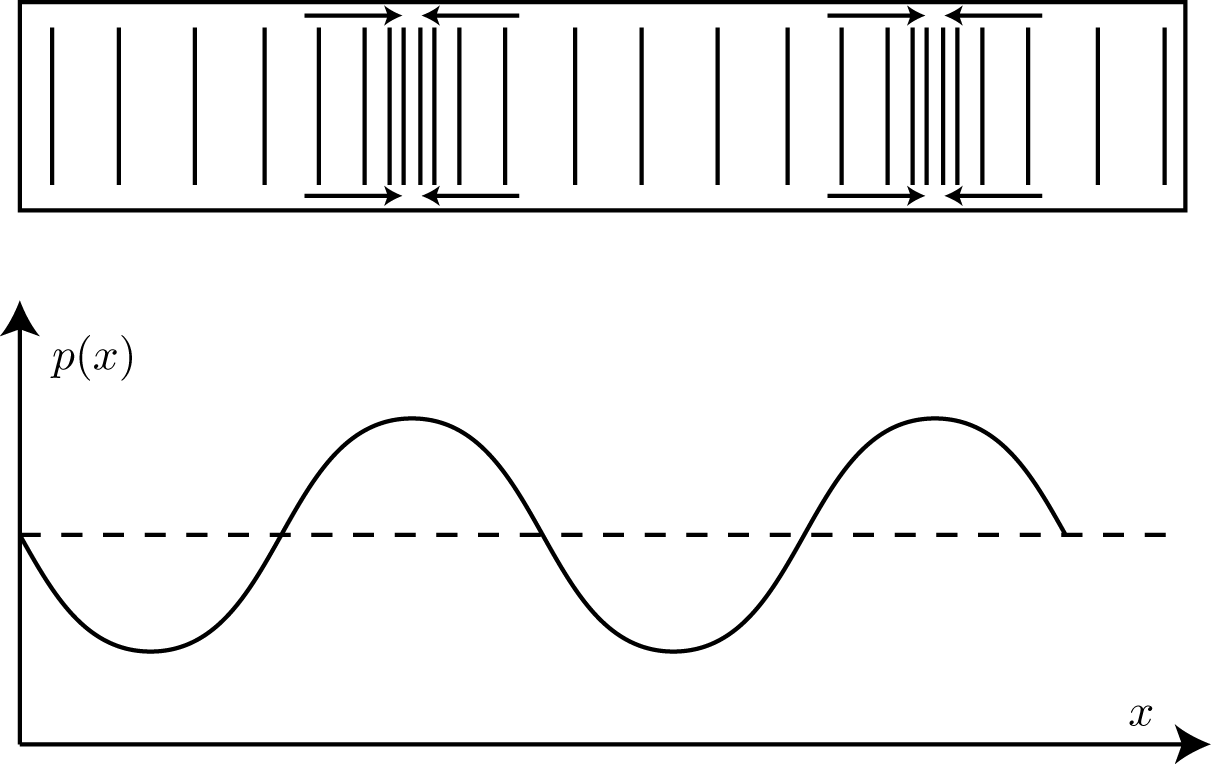
\includegraphics[width=0.7\linewidth]{skizzen/19/19B23}
\end{center}
Schwingungsknoten $ \hat{=} $ Druckband\\
Erinnerung: "Flammrohr", letzte L vor X-Mas 2015\\
Beispiel für stehende Schallwelle: Schwingungen der Luftsäule (z.B. Orgelpfeifen)
\begin{center}
	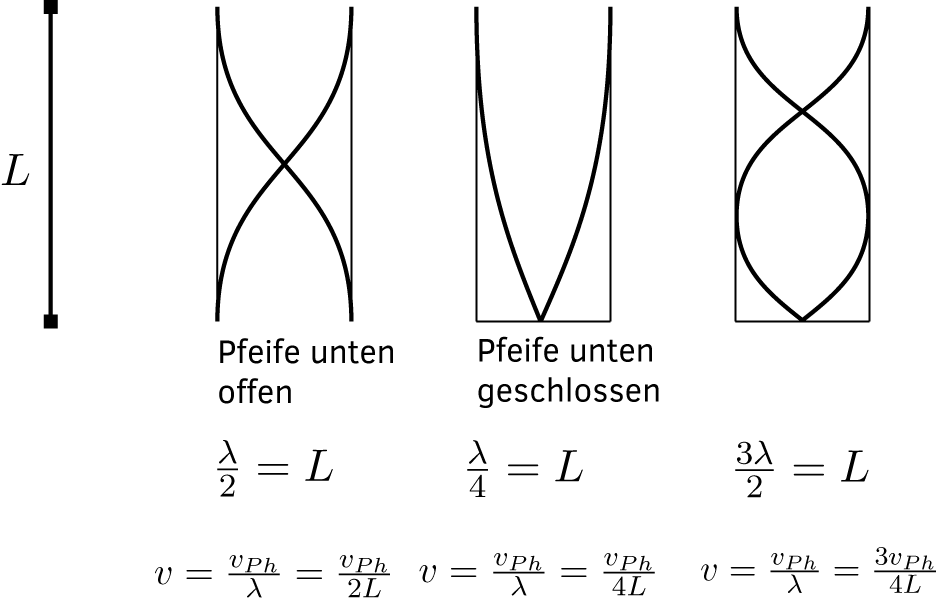
\includegraphics[width=0.7\linewidth]{skizzen/19/19B24}
\end{center}
Was bestimmt $ v_{Ph} $ von Schallwellen?\\
$ \Rightarrow $ Rücktreibende Kraft bei Druckschwankungen?\\
Seilwelle: $ \frac{\pi}{\rho} \Rightarrow \frac{d\overset{\text{Druck}}{p}}{d\rho}=v^2_{Ph}$\\
Bei adiabatischer Druckänderung  (kein Wärmeausgleich, schnell) folgt:\\
$$ \frac{dp}{d\rho} = \kappa \cdot \frac{K_B \cdot T}{m} \Rightarrow \boxed{v_{Ph} = \sqrt{\kappa\cdot\frac{K_BT}{m}}}$$\\
$ \Rightarrow $ Schallwellen sind dispersionsfrei (zum Glück)
$$ \omega = \v_{Ph} \cdot \kappa = \sqrt{\kappa\cdot\frac{K_BT}{m}} \cdot K $$
$ v_{Ph} = v_{Ph}(\kappa,T,m) $\\
Erinnerung: $ \kappa = 1 + \frac{2}{f} $ \hspace{5mm} $ f $: $ \# $ Freiheitsgrade des Moleküls\\
\enter
$ v_{Ph} $ @ 273K:\\
\begin{align*}
\text{Luft: } &N_2 \hspace{3mm}; m=28u; 2\text{-atomig}; f=5; \kappa = \frac{7}{5} \Rightarrow v_{Ph}=\SI{331}{\meter\per\second}\\
&H_2 \hspace{3mm}; m=2u; 2\text{-atomig}; f=5; \kappa = \frac{7}{5} \Rightarrow v_{Ph}=\SI{1240}{\meter\per\second} \\
\text{Helium: } &He \hspace{3mm}; m=4u; 1\text{-atomig}; f=3; \kappa = \frac{5}{3} \Rightarrow v_{Ph}=\SI{1007}{\meter\per\second}\\
&\omega= v_{Ph} \cdot K \Rightarrow \nu = \frac{v_{Ph}}{\lambda}
\end{align*}
Bei gleicher Geometrie (z.B. eines Resonators) ändert sich $ \nu $ bei Austausch des Gases: (Luft $ \rightarrow $ He : $ \nu \rightarrow \approx 3 \cdot \nu$)\\
\subsubsection{Experiment: Helium-stimme}\enter
Beachte: $ \nu = \frac{v_{Ph}(\sqrt{T})}{\lambda} $ : Temperatureinfluss auf "Stimmung" von Instrumenten \\
Vergleiche: $ \v_{Ph} $ und thermische Geschwindigkeit $ v_{th} $\\
\begin{align*}
&v_{Ph} = \sqrt{\kappa\frac{K_BT}{m}} &&; \sqrt{<v_{th}^2>} = \sqrt{3\frac{K}{m}}\\
\Rightarrow &\frac{v_{th}}{v_{Ph}}=\sqrt{\frac{3}{\kappa}} &&\Rightarrow v_{th} \approx 1,3 \cdot v_{Ph} ... 1,4 \cdot v_{Ph}\\
 v_{th}&  \text{ ist \underline{nicht }}  >>  v_{Ph} &&\Rightarrow \text{ kein schneller thermischer Ausgleich}\\
 & &&\Rightarrow \text{ Adiabatische Näherung ok!}
\end{align*}
\begin{center}
	\rule{5cm}{.2pt}
\end{center}
\subsubsection{Longitudinal Schallwellen in Festkörpern}\hfill\\
Wellengleichung: $ v_{Ph}^2 \cdot \frac{\partial^2\Psi}{\partial x^2} = \frac{\partial^2\Psi}{\partial t^2} $\\
Seilwelle: $ v_{Ph} = \sqrt{\frac{\tau}{\rho}} $\\
\subsubsection{Experiment: Schallwelle in Metallstab}
\enter
\begin{center}
	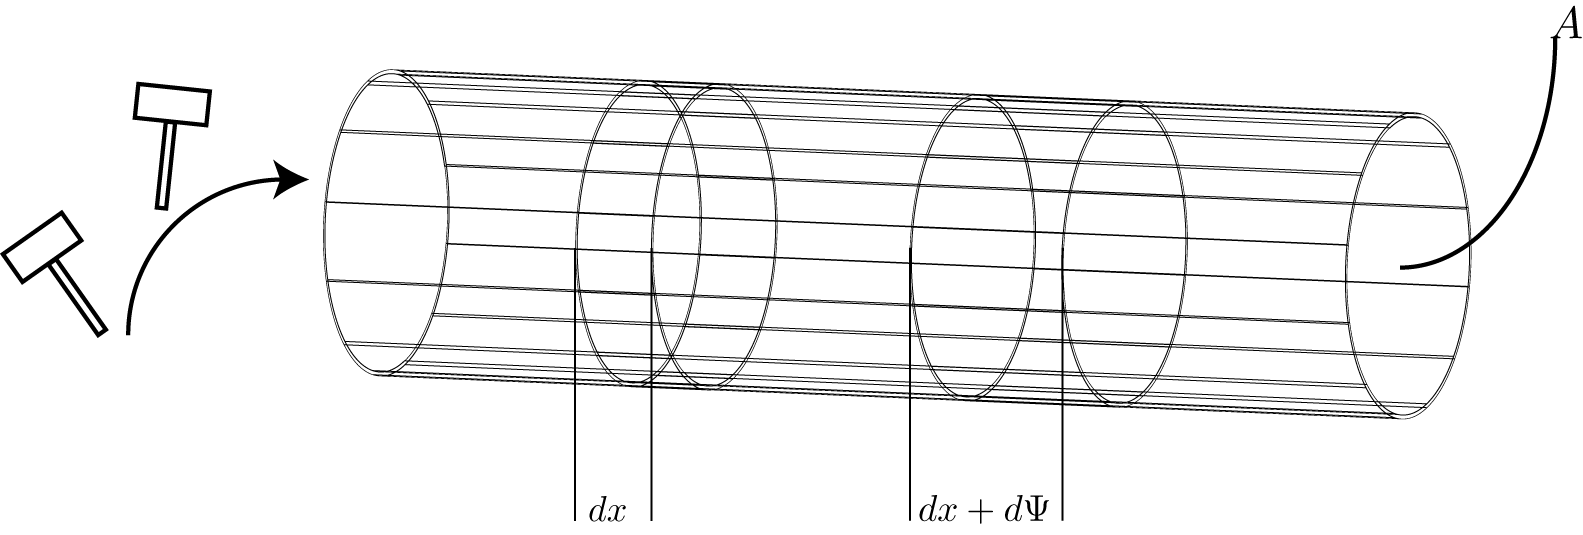
\includegraphics[width=0.7\linewidth]{skizzen/19/19B25}
\end{center}
Verformung von $ dx $ auf $ dx+x\Psi $\\
Dehnung: $ \epsilon = \frac{d\Psi}{dx} $\\
Verallgemeinerung Hook'sches Gesetz: $ \sigma = \frac{F}{A} = \underbracket{E}_{\mathclap{\text{Elasititätsmodul}}} \cdot \epsilon$\\
\begin{align*}
\rightarrow dF &= A \cdot E \cdot \frac{d\Psi}{dx}\\
\frac{dF}{dx} &= \underline{A \cdot E \cdot \frac{d^2\Psi}{dx^2}} \hspace{2cm} \text{(*)}
\end{align*}
\begin{align*}
\text{Beschleunigung auf Massenelement: }  dm = \rho\cdot dV = \rho\cdot A \cdot dx \\
dF = dm \cdot \frac{\partial^2\Psi}{\partial t^2} = \rho \cdot A \cdot dx \cdot \frac{\partial^2\Psi}{\partial t^2}\\
\frac{dF}{dx} = \rho \cdot A \cdot \frac{\partial^2\Psi}{\partial t^2} \hspace{2cm} \text{(**)}
\enter
\end{align*}
$$ \text{(*) (**) : } \boxed{\frac{E}{\rho} \cdot \frac{\partial^2\Psi}{\partial x^2} =  \frac{\partial^2 \Psi}{\partial t^2}} $$
\begin{center}
	Wellengleichung mit $ \underline{\underline{v_{Phi} = \sqrt{\frac{E}{\rho}}}} $ ; dispersionsfrei
\end{center}
$$ \underline{\underline{\omega = \sqrt{\frac{E}{\rho}} \cdot K}} $$
\begin{align*}
\text{Typische Werte (Stahl): } &E \approx \SI{2E11}{\newton\per\meter^2} \hspace{2cm} (200\si{\giga\pascal}) \\
&\rho = \SI{8E3}{\kilogram\per\meter^3}\\
\Rightarrow v_{Ph} = \sqrt{\frac{E}{\rho}} \approx \SI{5E3}{\meter\per\second} >> v_{Ph} \text{ (Luft)}
\end{align*}

In Festkörpern sind wegen Schwerkraft auch transversal Wellen Möglich: \hspace{2cm} $ G $ : Schermodul

$$ \underline{\underline{\Rightarrow v_{Ph} = \sqrt{\frac{G}{\rho}}}} $$